\section*{Introduction}
This paper looks at the incentives surrounding a particular program for allocating public infrastructure funds and determines if the program incentivizes conspicuous public spending.
For this, we define conspicuous public spending as allocating public spending to publicly salient projects that benefit the immediate interests of voters instead of publicly insignificant but necessary long-term infrastructure projects. 
Thus, conspicuous public spending is a trade-off between the voters' long-term and the politician's immediate interest in signaling competence to her voter base. 
To investigate conspicuous spending in politics, we exploit a program known as the Aldermanic Menu Program in the City of Chicago. 
The aldermanic menu program was initiated in 1994 and continues to this day \cite{OIGaudit}. 
The program delegates approximately \$ 66 million every year to be split equally amongst the 50 aldermen in Chicago's city council to be spent on projects their unilaterally select for their ward, given a ``menu'' of acceptable expenditures. 
However, ``off-menu'' expenditures are also allowed, of which most ``off-menu'' funds go towards Parks, Chicago Public Schools, and miscellaneous beautification projects such as trees, murals, decorative garbage cans, designer bike racks, and more\cite{OIGaudit}. 
While on-menu items are typically also provided by other funding sources within Chicago's Capital Improvement Program, off-menu items such as murals and statues usually are directly credited to the Aldermen, thus giving an incentive to ``pander.''  
The program is unique insofar that it gives elected politicians a wide berth over a significant portion of the City's infrastructure budget and allows its use for items that one does not typically think of as core infrastructure. 
An example of a portion of a menu from 2013 is shown below in figure 1.


\begin{figure}[H]
    \centering
    \caption{An Example of an Aldermanic Menu from 2012/2013}
    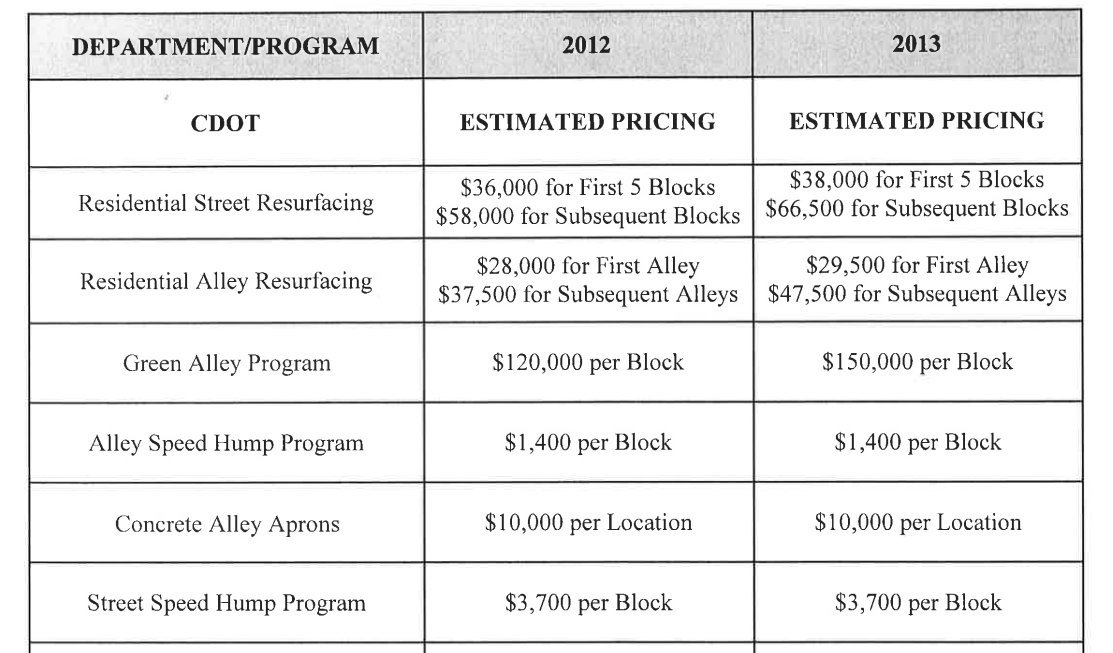
\includegraphics[scale=0.38]{input/menu_example.png}
\end{figure}

This paper's contribution to the literature will use the Aldermanic menu program to determine whether newer politicians with weaker electoral positions are more willing to engage in conspicuous spending, as indicated by spending more money on ``off-menu'' items that are typically items that more often directly credit the alderman for funding and creating. 
This paper employs a simple career concerns model of political budget allocations where a politician can spend money on long-term core infrastructure or on publicly salient spending to win reelection. 
This ``fake-it-till-you-make-it'' model comes with a few primary predictions: firstly, that ceteris-paribus that voters are more likely to reelect politicians who engage in more conspicuous expenditures, regardless of the harm it causes. 
Secondly, the model shows that the more experienced a politician is, the less they sacrifice voters' long-term interests since finding and implementing conspicuous public programs is more costly to politicians (in terms of time, effort, etc.) than programs that do not feature such a public element. 
In order to show that off-menu expenditures matter to voters, this paper exploits the multiple election periods to estimate the correlation between off-menu expenditures before an election and the Incumbent's election results and show that off-menu expenditures are significantly correlated with electoral performance, even when incorporating two-way fixed effects. 
Finally, we show an implication of this model that more experienced politicians do not engage in conspicuous expenditures to the same degree as newer politicians. 
We test this using differences-in-differences methods and regression discontinuity methods. 
Both methods show that newer alderpersons engage significantly off-menu spending by spending more on non-infrastructure items—however, the data and anecdotal information point toward a voter-selection effect rather than an electoral-incentive effect that our model presents. 


